\documentclass[letterpaper, 10 pt, conference]{cls/ieeeconf}
\IEEEoverridecommandlockouts
%\overrideIEEEmargins                                     
\let\proof\relax
\let\endproof\relax

\usepackage[table,usenames,dvipsnames]{xcolor}      % color
%\usepackage[shortlabels]{enumitem}
\usepackage[noadjust]{cite}
\usepackage{amsmath,amssymb,amsfonts,amsthm,dsfont,mathtools}
\usepackage{nicematrix}
\usepackage{comment}

\usepackage{adjustbox}
\usepackage{graphicx,tabularx,adjustbox,color}
\usepackage{pdfpages}
\usepackage{multirow}
\usepackage[font=footnotesize]{caption}
% \captionsetup[algorithm]{font=small}
\usepackage[font=footnotesize]{subcaption}

%\usepackage{float}
%\usepackage{subfig}


\usepackage{algorithmic}
\usepackage[ruled,vlined]{algorithm2e}
\usepackage{stackengine}
\def\delequal{\mathrel{\ensurestackMath{\stackon[1pt]{=}{\scriptstyle\Delta}}}}
%\usepackage{dirtytalk}
\allowdisplaybreaks
\renewcommand{\baselinestretch}{.985}
%\usepackage[style=numeric, maxbibnames=9]{biblatex}
%\addbibresource{./bib/ref.bib}

\usepackage[breaklinks=true, colorlinks, bookmarks=true, citecolor=Black, urlcolor=Violet,linkcolor=Black]{hyperref}



%\usepackage[square,sort,comma,numbers]{natbib}
%\usepackage{graphicx}https://www.overleaf.com/project/606b49686686d6a38c5166b3
%\usepackage{textcomp}
%\usepackage{xcolor}1
%\usepackage{subfigure}
%\usepackage{enumerate,url}
%\usepackage{natbib}
%\usepackage{geometry}
%\usepackage{indentfirst}
%\setlength{\parindent}{2em}
%\usepackage[utf8]{inputenc}



% Commands
\newcommand{\prl}[1]{\left(#1\right)}
\newcommand{\brl}[1]{\left[#1\right]}
\newcommand{\crl}[1]{\left\{#1\right\}}
\newcommand{\norm}[1]{\left\lVert#1\right\rVert}
\newcommand{\Int}{\operatorname{Int}}
\newcommand{\scaleLine}[2][1]{\resizebox{#1\linewidth}{!}{#2}}
\newcommand{\scaleMathLine}[2][1]{\resizebox{#1\linewidth}{!}{$\displaystyle{#2}$}}
\DeclareMathOperator*{\diag}{diag}
\DeclareMathOperator*{\argmin}{arg\,min}

% Environments
%\newtheorem{proposition}{Proposition}
%\newtheorem{lemma}{Lemma}
%\newtheorem{theorem}{Theorem}
%\theoremstyle{definition}
%\newtheorem{definition}{Definition}
%\newtheorem*{problem*}{Problem}
%\newtheorem{problem}{Problem}
%\newtheorem*{remark*}{Remark}

\newtheorem{theorem}{Theorem}[section]
\newtheorem{proposition}[theorem]{Proposition}
\newtheorem{lemma}[theorem]{Lemma}
\newtheorem{Assumption}[theorem]{Assumption}
\newtheorem{corollary}[theorem]{Corollary}
\theoremstyle{remark}
\newtheorem{remark}[theorem]{Remark}
\theoremstyle{definition}
\newtheorem{definition}[theorem]{Definition}
\newtheorem{problem}{Problem}
\newtheorem*{problem*}{Problem}
\newtheorem{method}[]{Procedure}
\theoremstyle{definition}


% Comments:
\newcommand{\TODO}[1]{{\color{red}#1}}
\newcommand{\KL}[1]{$\clubsuit$\footnote{\TODO{Kehan}: #1}}
\newcommand{\NA}[1]{$\spadesuit$\footnote{\TODO{Nikolay: #1}}}

%%%%%%%%%%%%%%%%%%%%%%%%%%%%%%%%%%%%%%%%%%%%%%%
\input{cls/sym.tex}
%%%%%%%%%%%%%%%%%%%%%%%%%%%%%%%%%%%%%%%%%%%%%%%



\title{\LARGE \bf Safe Stabilizing Control for Polygonal Robots in Dynamic Elliptical Environments} 

%%%%% title candidates
% Safe autonomy of Rigid-Body robots in dynamical elliptical environments with Control Barrier Functions


\author{Kehan Long \qquad Khoa Tran \qquad Melvin Leok \qquad Nikolay Atanasov
%  
% \thanks{We gratefully acknowledge support from ...}%
% %
\thanks{The authors are with the Contextual Robotics Institute, University of California San Diego, La Jolla, CA 92093, USA (e-mails: {\tt\small \{k3long,\allowbreak k2tran,\allowbreak mleok,\allowbreak natanasov\}@ucsd.edu}).}%
}


\begin{document}
\maketitle
% \setlength{\abovedisplayskip}{0.1cm}
% \setlength{\belowdisplayskip}{0.2cm}
\begin{abstract}
This paper addresses the challenge of safe navigation for rigid-body mobile robots in dynamic environments. We introduce an analytic approach to compute the distance between a polygon and an ellipse, and employ it to construct a control barrier function (CBF) for safe control synthesis. Existing CBF design methods for mobile robot obstacle avoidance usually assume point or circular robots, preventing their applicability to more realistic robot body geometries. Our work enables CBF designs that capture complex robot and obstacle shapes. We demonstrate the effectiveness of our approach in simulations highlighting real-time obstacle avoidance in constrained
and dynamic environments for both mobile robots and multi-joint robot arms. 
%bridges this gap by leveraging the proposed analytic distance computation to handle more complex robot and obstacle shapes. We demonstrate the effectiveness of our approach through numerical simulations, highlighting real-time obstacle avoidance capabilities in tight and dynamic environments for both ground robots and multi-link robot arms. 
\end{abstract}

\section{Introduction}
\label{sec:intro}

\subsection{Motivation}

Reliable estimation of a signal (or image) from nonlinear observations is of fundamental interest to several signal processing and machine learning applications. However, such an estimation is confounded by cases where the nonlinearity in each observation is well-modeled by a \emph{periodic} function such as a sinusoidal function, or sawtooth function, or a square-wave function. Periodic functions are many-to-one mappings, and inverting them can be challenging.

Our focus in this paper is a special kind of periodic nonlinear observation model encountered in high-dynamic range (HDR) imaging. It is well known that real world scenes contain a large range of brightness levels. However, due to hardware limitations, not all brightness levels can be accurately captured using conventional photography; if tuned incorrectly, most scene intensity levels can lie in the saturation region of the image sensors, causing loss of scene information. Similar problems arise in the case of multiplexed imaging systems, such as lensless and coded aperture imaging~\cite{codedaperture,asif2017flatcam}.

%While increasing the dynamic range can solve this problem, it is an impractical strategy since imaging sensors need to have infinite dynamic range, which is infeasible. 
One solution is to increase the dynamic range of the image sensors, but this can lead to expensive hardware. An alternative solution is to deploy a special type of image sensor that {wraps} the observed intensity value at a pixel over a given dynamic range. This is analogous to the familiar \emph{modulo} operation with respect to a parameter $R$, and we call this stylized imaging system a \emph{modulo camera}~\cite{ICCP15_Zhao}.  
Fig.~\ref{fig:func}(a) (black) depicts the modulo nonlinearity, and a major challenge is to undo the effect of this transformation for each observed pixel.

An added challenge in HDR imaging arises due to \emph{quantization}. In fact, the ``true" observations in a modulo camera are quantized versions of the (idealized) modulo observation, and the errors caused in the quantization propagates into the estimation process. Loss of information in the quantization process is unavoidable in principle, and the effect of quantization is magnified with fewer quantization levels. In acquisition systems with low bit-depth, such estimation errors can be very pronounced. Fig.~\ref{fig:func}(a) (cyan) depicts the quantization nonlinearity incurred during the observation process.

\subsection{Setup}

We formalize the above discussion as follows. Assume $\mathcal{X} \subseteq \R^{n}$ to be a given (known) subset in the data space, and consider a signal (or image) $x \in \mathcal{X}$. We model (possible) multiplexing operations and gain adjustments as linear transformations, denoted by $A\in\mathbb{R}^{p\times n}$ and $C\in\R^{m\times p}$ respectively. The composite observation model becomes:
\begin{equation}
\label{quan_obs}
u=f(Ax),~y=Q(Cu),
\end{equation}
where $f(\cdot)=\mod(\cdot,R)$ denotes the modulo function with respect to a range parameter $R$ and $Q(\cdot)$ denotes a quantization function. In this paper, we consider a 1-bit quantization function with only two levels, $0$ and $1$. A representative example is shown in Fig.\ \ref{fig:func} where $A$ and $C$ are identity operators. In  Figs~\ref{fig:func}(c)  and~\ref{fig:func}(d), the outputs of the functions $f$ and $Q$ are displayed when a test grayscale image (Fig.\ \ref{fig:func}(a)) is used in the input. Our overall objective is to estimate the original signal $x$ from the set of measurements $y$. 

%%%%%%%%%%%%%%%%%%%%%%%%%%%%%%%%%%%%%
\begin{figure}[t]
	
	\begin{center}
		\begingroup
		\setlength{\tabcolsep}{0.1pt} % Default value: 6pt
		\renewcommand{\arraystretch}{.1} % Default value: 1
		\begin{tabular}{ccc}      %{c@{\hskip .1pt}c@{\hskip .1pt}c}
			\multicolumn{3}{c}{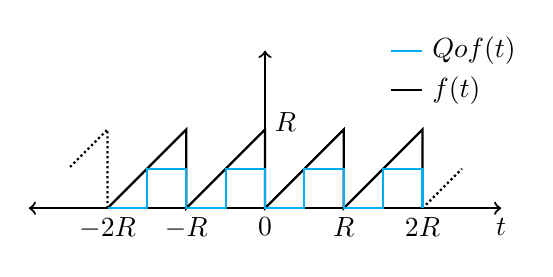
\begin{tikzpicture}
				\draw[<->,thick] (-3,0)--(3,0) node[anchor=north]{$t$};
				\draw (0,0) node[anchor=north]{$0$};
				\draw (0,1.1) node[anchor=west] {$R$};
				\draw (1,0) node[anchor=north]{$R$};
				\draw (2,0) node[anchor=north] {$2R$};
					\draw (-1,0) node[anchor=north]{$-R$};
				\draw (-2,0) node[anchor=north] {$-2R$};
				\draw[] (2,2) node[anchor=west] {{$Qof(t)$}};
				\draw[cyan,thick] (1.6,2) -- (2,2);
				%\draw [densely dotted,thick] (-2.5,1)--(3,1);
				\draw[->,thick] (0,0)--(0,2);
				\draw[] (2,1.5) node[anchor=west] {{$f(t)$}};
				\draw[thick] (1.6,1.5) -- (2,1.5);
				\draw[thick] (-2,0) --(-1,1)-| (-1,0) -- (0,1) -| (0,0) --(1,1)-| (1,0) -- (2,1) -| (2,0);
				\draw[densely dotted,thick] (2,0)--(2.5,0.5);
				\draw[densely dotted,thick] (-2,0)|-(-2,1) -- (-2.5,0.5);
				\draw[thick, cyan] (-2,0) -- ++(0.5,0)-| ++(0,0.5) -- ++(0.5,0) -| ++(0,-0.5) -- ++(0.5,0)-| ++(0,0.5) -- ++(0.5,0) -| ++(0,-0.5) -- ++(0.5,0)-| ++(0,0.5) -- ++(0.5,0) -| ++(0,-0.5) -- ++(0.5,0)-| ++(0,0.5) -- ++(0.5,0) -| ++(0,-0.5);
				\end{tikzpicture}}\\
			\multicolumn{3}{c}{(a)}\\
			\includegraphics[trim = 10mm 60mm 25mm 40mm,clip, width = 0.32\linewidth]{./orgimg.pdf}&
			\includegraphics[trim = 10mm 60mm 25mm 40mm,clip, width = 0.32\linewidth]{./modimg.pdf}&
			\includegraphics[trim = 10mm 60mm 25mm 40mm,clip,width = 0.32\linewidth]{./quantimg.pdf} \\
			(b) & (c) & (d)
		\end{tabular}
		\endgroup
	\end{center}
	\caption{\small{\emph{ (a) Modulo function, $f(t) = \mod(t,R)$ and quantized modulo function, $Qof(t)$; (b,c,d) Depiction of forward model. An input image (b) is transformed via a modulo function $f(t) = \mod(t,R)$, to (c). Such a ``modulo" image is further quantized to obtain (d).}}}
	\label{fig:func}
\end{figure}
%%%%%%%%%%%%%%%%%%%%%%%%%%%%%%%%%%%%%%%%%%%%%%%%%%

\subsection{Our contributions}

Clearly, the above estimation procedure is challenging due to the highly non-invertible nature of the observation model. In this paper, we design a systematic approach that takes some initial steps towards resolving this challenge. Our overarching assumption is that the measurement operations $A$ and $C$ are part of the design space. The core idea in our approach is that a very small, but carefully designed, non-adaptive set of measurements can support efficient estimation of the unknown signal.

Our approach follows stagewise. First, we consider the problem of inverting the quantization function, i.e., recovering $u$ from $y = Q(Cu)$. We demonstrate the existence of a linear operator $C$ (together with an efficient reconstruction algorithm) that supports such an inversion. Specifically, our operator $C$ obeys a particular block-diagonal form with weights chosen according to a harmonic progression; see Section~\ref{sec:Model} for details. We only consider 1-bit quantization functions, but similar ideas can presumably be extended for a higher number of quantization levels. In addition, our method supports the criterion of \emph{consistent reconstruction} as defined in \cite{jacques2011dequantizing}.

Next, we consider the problem of inverting the modulo operation, i.e., recovering $x$ from $u = f(Ax)$.  We propose an algorithm that builds upon the approach proposed in \cite{SoltaniHegde_ICASSP16}. In particular, we show that if the operator $A$ satisfies a certain \emph{factorization} $A = DB$, then $f$ can be stably inverted. To enable efficient inversion, the matrix $D$ must also be block-diagonal with weights chosen either randomly, or according to a geometric progression. In the former case, the reconstruction algorithm is an extension of the approach of~\cite{SoltaniHegde_ICASSP16}, while in the latter case the reconstruction follows the approach of~\cite{ICCP15_Zhao}.

The above two-stage procedure can be easily adapted to the case where we have some prior knowledge of the original signal $x$. This enables our approach to be used in conjunction with compressive imaging architectures. Common priors used in compressive imaging include \emph{sparsity} in some known orthonormal basis~\cite{foucart2013}. Note that our measurements are highly quantized and the total ``bit" complexity of our observations is far smaller than conventional techniques. Therefore, within our framework, one can choose to increase the number of quantizer measurements (rows of $C$) and/or modulo measurements (rows of $D$) in order to achieve better estimation performance.


Fig.~\ref{fig:demo} displays some representative results using our approach. We begin with a standard ``Peppers" image, compute a modulo transformation with three multiplexed measurements per pixel, and further modulate it with a sequence of three harmonic multipliers per measurement before passing it through a 1-bit quantizer. (In words, the overall ``oversampling factor" in our method is $9\times$.) The final binary measurements displayed in Fig.\ \ref{fig:demo}(a) are given as inputs to our reconstruction algorithm. The results from the first and second stages are displayed as images in Fig.\ \ref{fig:demo}(b). As is visually evident, our method is able to successfully reconstruct the image, as displayed in Fig.\ \ref{fig:demo}(c). 


\begin{figure}[t]
	\begin{center}
		\begingroup
		\setlength{\tabcolsep}{1pt} % Default value: 6pt
		\renewcommand{\arraystretch}{.1} % Default value: 1
		{\setlength{\tabcolsep}{1mm}
		\begin{tabular}{ccc|c|c}      %{c@{\hskip .1pt}c@{\hskip .1pt}c}
			\centering
			\includegraphics[trim = 30mm 60mm 40mm 65mm,clip, width = 0.15\linewidth]{./quant11.pdf}&
			\includegraphics[trim = 30mm 60mm 40mm 65mm,clip, width = 0.15\linewidth]{./quant12.pdf}&
			\includegraphics[trim = 30mm 60mm 40mm 65mm,clip, width = 0.15\linewidth]{./quant13.pdf}&
			\includegraphics[trim = 90mm 125mm 90mm 120mm,clip, width = 0.18\linewidth]{./mod11.pdf}&
				\multirow{3}{20mm}{\includegraphics[trim = 90mm 85mm 90mm 120mm,clip, width = \linewidth]{./dms_img.pdf}}\\
			\includegraphics[trim = 30mm 60mm 40mm 65mm,clip, width = 0.15\linewidth]{./quant21.pdf}& 
			\includegraphics[trim = 30mm 60mm 40mm 65mm,clip, width = 0.15\linewidth]{./quant22.pdf}&
			\includegraphics[trim = 30mm 60mm 40mm 65mm,clip, width = 0.15\linewidth]{./quant23.pdf}&
			\includegraphics[trim = 90mm 125mm 90mm 120mm,clip, width = 0.18\linewidth]{./mod21.pdf}&\\
			\includegraphics[trim = 30mm 50mm 40mm 65mm,clip, width = 0.15\linewidth]{./quant31.pdf}& 
			\includegraphics[trim = 30mm 50mm 40mm 65mm,clip, width = 0.15\linewidth]{./quant32.pdf}&
			\includegraphics[trim = 30mm 50mm 40mm 65mm,clip, width = 0.15\linewidth]{./quant33.pdf}& 
			\includegraphics[trim = 90mm 125mm 90mm 120mm,clip, width = 0.18\linewidth]{./mod31.pdf}&\\[1pt]
			\multicolumn{3}{c|}{(a)} &(b)&{\centering(c)}
		\end{tabular}}
		\endgroup
	\end{center}
	\caption{\small{\emph{Illustration of our approach. A given input image is modulated pixel-wise with three pre-chosen weights, passed through a modulo sensor, modulated again pixel-wise with three weights, and quantized to binary images. The resulting observations are shown in (a). The images in (b) and (c) represent the reconstruction of the modulo images, $\widehat{u}$ and the final image, $\widehat{x}$, respectively.}}}
	
	\label{fig:demo}
\end{figure}



%\section{Related Work}
\label{sec: relate_work}

Obstacle avoidance, in both static and dynamic environments, has persistently been a central issue in robotics. Over the years, various algorithms and methodologies have been proposed to address this challenge.

At the planning level, several motion planning algorithms have been developed to provide a feasible path that ensures obstacle avoidance, including prominent approaches like $\textbf{A}^*$~\cite{A_star_planning},$\textbf{RRT}^*$~\cite{RRT_star}, and their variants~\cite{informed_rrt_star, neural_rrt_star}. However, those approaches typically assume the existence of a low-level tracking controller and may not be applicable in dynamic environments. and may not be applicable in dynamic environments. A significant contribution to the field was made by Khatib~\cite{potential-field}, who introduced artificial potential fields to enable collision avoidance during not only the motion planning stage but also the real-time control of a mobile robot. Later, Rimon and Koditschek \cite{navigation-function} developed navigation functions, a particular form of artificial potential functions. These functions strive to ensure collision avoidance and stabilization towards a goal configuration simultaneously. 
% Meanwhile, Fox \cite{Fox1997TheDW} introduced the dynamics window concept, an influential approach to obstacle avoidance that proactively filters out unsafe control actions. 
In recent years, research has delved into the domain of trajectory generation and optimization, with innovative algorithms proposed for quadrotor safe navigation~\cite{mellinger_snap_2011, zhou2019robust, tordesillas2019faster}. In parallel, the rise of learning-based approaches~\cite{michels2005high, pfeiffer2018reinforced, loquercio2021learning} has added a new direction to the field, utilizing machine learning to facilitate both planning and real-time obstacle avoidance. Despite their promise, these methods often face challenges in dynamic environments and in providing safety guarantees.


In the field of safe control synthesis, integrating control Lyapunov functions (CLFs) and control barrier functions (CBFs) into a quadratic program (QP) has proven to be a reliable and efficient strategy for formulating safe stabilizing controls across a wide array of robotic tasks~\cite{glotfelter2017nonsmooth, grandia_2021_legged, wang2017_aerial}. While CBF-based methodologies have been deployed for obstacle avoidance~\cite{srinivasan2020synthesis, Long_learningcbf_ral21, almubarak2022safety, dawson2022learning, abdi2023safe}, such strategies typically simplify the robot as a point or circle and assume static environments when constructing CBFs for control synthesis. Some recent advances have also explored the use of time-varying CBFs to facilitate safe control in dynamic environments~\cite{he2021rule, molnar2022safety, hamdipoor2023safe}. However, this concept has yet to be thoroughly investigated in the context of obstacle avoidance for rigid-body robots. For the safe autonomy of robot arms, Koptev \textit{et al}.\cite{Koptev2023_neural_joint_control} introduced a neural network approach to approximate the signed distance function of a robot arm and use it for safe reactive control in dynamical environment. 




Researchers~\cite{ding2022configurationaware} proposed a configuration-aware control approach for the robot arm by integrating geometric restrictions with Control Barrier Functions. 



Mostly related to our work, Thirugnanam \textit{et al}. \cite{discrete_polytope_cbf} introduced a discrete CBF constraint between polytopes and further incorporated the constraint in a model predictive control framework to enable safe navigation. The authors \cite{polytopic_cbf} also extended the formulation for continuous-time systems but the CBF computation between polytopes still remained numerical, requiring a duality-based formulation with non-smooth CBFs. 




\textbf{Contributions}: 1) We present an analytic distance formula in $SE(2)$ for elliptical and polygonal objects, enabling closed-form calculations for distance and its gradient. 2) We introduce a novel time-varying control barrier function tailored for robots described by one or multiple $SE(2)$ configurations based on the analytic distance. Its efficacy is validated through applications in ground robot navigation and multi-link robot arm demonstrations.













\section{Problem Formulation}\label{sec:problem}

%\subsection{Notations}
% \footnotetext[1]{\textbf{Notation. }
% The sets of non-negative real and natural numbers are denoted $\bbR_{\geq 0}$ and $\bbN$. For $N \in \bbN$, $[N] := \{1,2, \dots N\}$. The orientation of a 2D body is denoted by $0 \leq \theta < 2\pi$ for counter-clockwise rotation. We denote the corresponding rotation matrix as 
% % \begin{equation}
% % \label{eq: rotation}
%     $\bfR(\theta) = \begin{bmatrix} \cos \theta & -\sin \theta \\ \sin \theta & \cos \theta \end{bmatrix}.$
% % \end{equation
% The $L_2$ norm for a vector $\bfx$ is denoted by $\|\bfx\|$. The gradient of a differentiable function $V$ is denoted by $\nabla V$, and its Lie derivative along a vector field $f$ by $\calL_f V  = \nabla V \cdot f$. A continuous function $\alpha: [0,a)\rightarrow [0,\infty )$ is of class $\calK$ if it is strictly increasing and $\alpha(0) = 0$. A continuous function $\alpha:\mathbb{R} \rightarrow \mathbb{R}$ is of extended class $\calK_{\infty}$ if it is of class $\calK$ and $\lim_{r \rightarrow \infty} \alpha(r) = \infty$.}

% \NA{The footnote should be referenced somewhere. It might be better to just introduce the notation in the main text whenever it is needed.}

Consider a robot with dynamics governed by a non-linear control-affine system,
%
\begin{equation}
\label{eq: dynamic}
\begin{aligned}
    &\dot{\bfx} = f(\bfx) + g(\bfx) \bfu ,
\end{aligned}
\end{equation}
%
where $\bfx \in \calX \subseteq \mathbb{R}^{n}$ is the robot state and $\bfu \in  \mathbb{R}^{m}$ is the control input. Assume that $f : \mathbb{R}^{n} \mapsto \mathbb{R}^{n}$ and $g : \mathbb{R}^{n} \mapsto \mathbb{R}^{n \times m}$ are continuously differentiable functions. We assume the robot operates in a 2D workspace with a state-dependent shape $S(\bfx) \subset \bbR^2$. 


% \NA{Move this paragraph later, now that we define the robot shape $S(\bfx)$, it is not necessary to define the polygon here. It may be better to use a different letter than $S$ since (a) we use calligraphic fonts for sets and (b) we are defining $\calS$ as the safe region. One idea is to define $\calS(\bfx)$ as the robot shape and $\calF$ as the free space.}

We assume the $\bbR^2$ workspace is partitioned into a closed safe (free) region $\mathcal{F}(t)$ and an open unsafe region $\mathcal{O}(t)$ such that  $\mathcal{F}(t) \cap \mathcal{O}(t) = \emptyset$ and $\bbR^2 = \mathcal{F}(t) \cup \mathcal{O}(t)$. We assume the unsafe set $\mathcal{O}(t)$ is characterized by a collection of dynamical elliptical obstacles with known rigid-body motions, denoted as $\{\calE(\bfq_i(t), \bfR(\theta_i(t)), a_i, b_i)\}_{i=1}^N$. Here, $\bfq_i$ denotes the center of mass and $\bfR_i$ denotes the rotation matrix of the ellipse. In its body-fixed frame, $a_i$ and $b_i$ are the lengths of the semi-axes of the ellipse along the $x$-axis and $y$-axis, respectively.

\begin{problem*}
Given a robot with shape $S(\bfx)$ governed by dynamics \eqref{eq: dynamic} that can perfectly determine its state, the objective is to stabilize the robot safely within a goal region $\calG \subset \bbR^2$ such that $S(\bfx(t)) \cap \calO(t) = \emptyset$ for all $t \in \bbR_{\geq 0}$.
\end{problem*}



% In this section we review some notation and preliminaries on distributionally robust chance-constrained programming, control Lyapunov and barrier functions, and their use in systems with uncertainty

% \subsection{Control Lyapunov Function}
% The notion of a control Lyapunov function (CLF) was introduced in \cite{Artstein1983StabilizationWR, SONTAG1989117} to verify the stabilizability of control-affine systems \eqref{eq: dynamic}. Specifically, a (exponentially stabilizing) CLF $V: \calX \mapsto \bbR$ is defined as follows,
% %
% \begin{definition}
% A function $V \in \mathbb{C}^1(\calX,\mathbb{R})$ is a \emph{control Lyapunov function (CLF)} on $\calX$ for system \eqref{eq: dynamic} if $V(\bfx)>0, \forall \bfx \in \calX \setminus \{\boldsymbol{0} \}, V(\boldsymbol{0}) = 0$, and it satisfies:
% %
% \begin{equation}\label{eq: clf}
%     \inf_{\bfu \in \bbR^m} \text{CLC}(\bfx,\bfu) \leq 0, \quad \forall \bfx \in \calX,
% \end{equation}
% %
% where $\text{CLC}(\bfx,\bfu) := \mathcal{L}_f V(\bfx) + \mathcal{L}_g V(\bfx)\bfu + \alpha_V( V(\bfx))$
% is the \emph{control Lyapunov condition} (CLC) defined for some class $K$ function $\alpha_V$.
% \end{definition}


% \subsection{Control Barrier Function}

% To facilitate safe control synthesis, we consider a \textcolor{blue}{time-varying set $\calC(t)$} defined as the super zero-level set of a continuously differentiable function $h: \calX \times \bbR \mapsto \bbR$:
% %
% \begin{equation}
% \label{eq: safe_set}  
%     \calC(t) := \{\bfx \in \calX \subseteq \bbR^n: h(\bfx, t) \geq 0 \}.
% \end{equation}
% %
% Safety of the system \eqref{eq: dynamic} can then be ensured by keeping the state $\bfx$ within the safe set $\calC(t)$.

% \begin{definition}
% \label{def: tv_cbf}
% A function $h: \mathbb{R}^n \times \bbR_{\geq 0} \mapsto {\mathbb{R}}$ is a valid time-varying \emph{control barrier function (CBF)} on $\mathcal{X} \subseteq \mathbb{R}^n$ for \eqref{eq: dynamic} if there exists an extended class $\mathcal{K}_{\infty}$ function $\alpha_h$ with:
% %
% \begin{equation}\label{eq:tv_cbf}
%     \sup_{\bfu\in \mathcal{U}} \text{CBC}(\bfx,\bfu, t) \geq 0, \quad \forall \; (\bfx,t) \in \calX \times \bbR_{\geq 0},
% \end{equation}
% where the \emph{control barrier condition (CBC)} is:
% \begin{equation}
% \label{eq:tvcbc_define}
% \begin{aligned}
%     &\text{CBC}(\bfx,\bfu, t) := \dot{h}(\bfx, t) + \alpha_h(h(\bfx,t)) \\
%     & = \mathcal{L}_f h(\bfx, t) + \mathcal{L}_g h(\bfx, t)\bfu + \frac{\partial h(\bfx,t)}{\partial t} + \alpha_h(h(\bfx,t)).
% \end{aligned}
% \end{equation}
% \end{definition}


% % \textcolor{blue}{Note that the above definition assumes that the TV-CBF depends only first order in time explicitly. If $h$ has a higher order time dependency, we would need to modify \eqref{eq:tvcbc_define} to include higher order time derivatives.}

% Definition~\ref{def: tv_cbf} allows us to consider the following set of control values that render the safe set $\calC$ forward invariant, 
% \begin{equation}
% \label{eq: safe_control_set}
%     K_{\text{CBF}}(\bfx, t) := \left \{  \bfu \in \calU: \text{CBC}(\bfx,\bfu, t) \geq 0 \right \}. 
% \end{equation}

% % \begin{lemma}
% % \label{lemma: 1}
% % Suppose $\alpha: \bbR_{\geq 0} \mapsto \bbR_{\geq 0}$ is a locally Lipschitz continuous class $\calK$ function and $\eta : [t_0, t_1] \mapsto \bbR$ is an absolutely continuous function. If $\dot{\eta}(t) \geq - \alpha(\eta(t))$ for every $t \in [t_0, t_1]$, and $\eta(t_0) \geq 0$, then $\eta(t) \geq 0$ for all $t \in [t_0, t_1]$.
% % \end{lemma}

% % \begin{theorem}
% % \label{theorem: tv_cbc_validity}
% % Assume that $\bfu(\bfx, t) \in K_{\text{CBF}}(\bfx, t)$ is locally Lipschitz continuous in $\bfx$ and piecewise continuous in $t$ and that the unique solutions to \eqref{eq: dynamic} are defined over $[t_0, t_1]$. Then, if $h(\bfx, t)$ is a valid time-varying control barrier function, the set $\calC(t)$ is forward invariant under the control law $\bfu(\bfx, t)$.

% % \begin{proof}
% % We start by assuming that $\bfx(t_0) \in \calC(t_0)$, which implies that $h(\bfx(t_0), t_0) \geq 0$. Given that $h(\bfx, t)$ is a valid TV-CBF and hence $\bfu(\bfx, t) \in K_{\text{CBC}}(\bfx, t) \neq \emptyset$ results in a solution $\bfx$ to \eqref{eq: dynamic} with initial condition $\bfx(t_0)$ that satisfies $\dot{h}(\bfx(t), t) \geq -\alpha_h(h(\bfx(t), t))$ for all $t \in [t_0, t_1]$. Note that the solution $\bfx : [t_0, t_1] \mapsto \mathbb{R}^n$ exists by assumption. We then set $\eta(t) := h(\bfx(t), t)$. Applying Lemma~\ref{lemma: 1}, we deduce that $\eta(t) \geq 0$ for all $t \in [t_0, t_1]$. Hence, $\calC(t)$ is forward invariant, since $h(\mathbf{x}(t), t) \geq 0$ leads to $\bfx(t) \in \calC(t)$.

% % \end{proof}
% % \end{theorem}


% % %
% % Theorem.~\ref{theorem: tv_cbc_validity} implies that if there exists a TV-CBF for \eqref{eq: dynamic}, then the robot state evolves within the safe set $\calC(t)$ under a locally Lipschitz control law $\bfk(\bfx, t) \in K_{\text{CBF}}(\bfx, t)$.


% Suppose we are given a baseline feedback controller $\bfu = \bfk(\bfx)$ for the control-affine systems \eqref{eq: dynamic}, and we aim to ensure the safety and stability of the system.  \textcolor{blue}{By observing that both the CLC and CBC constraints are affine in the control input $\bfu$, a quadratic program (QP) can be formulated for online synthesis of a safe stabilizing controller for \eqref{eq: dynamic}:
% %
% \begin{equation}
% \begin{aligned}
% \label{eq: clf_cbf_qp}
%     \bfu(\bfx) = &\argmin_{\bfu \in \bbR^m,\delta \in \bbR} \| \bfu - \bfk(\bfx)\|^2 + \lambda \delta^2,  \\
%     \mathrm{s.t.} \, \,  &\text{CLC}(\bfx,\bfu) \leq \delta,  \text{CBC}(\bfx,\bfu, t) \geq 0,
% \end{aligned}
% \end{equation}
% %
% where $\delta \geq 0$ denotes a slack variable that relaxes the CLF constraints to ensure the feasibility of the QP, controlled by the scaling factor $\lambda > 0$.}

















\section{Preliminaries}
\label{sec: prelim}

In this section, we review preliminaries on control Lyapunov and barrier functions and discuss their use in synthesizing a safe stabilizing controller for dynamics in~\eqref{eq: dynamic}.

\subsection{Control Lyapunov Function}
The notion of a control Lyapunov function (CLF) was introduced in \cite{Artstein1983StabilizationWR, SONTAG1989117} to verify the stabilizability of control-affine systems \eqref{eq: dynamic}. Specifically, a (exponentially stabilizing) CLF $V: \calX \mapsto \bbR$ is defined as follows,
%
\begin{definition}
A function $V \in \mathbb{C}^1(\calX,\mathbb{R})$ is a \emph{control Lyapunov function (CLF)} on $\calX$ for system \eqref{eq: dynamic} if $V(\bfx)>0, \forall \bfx \in \calX \setminus \{\boldsymbol{0} \}, V(\boldsymbol{0}) = 0$, and it satisfies:
%
\begin{equation}\label{eq: clf}
    \inf_{\bfu \in \bbR^m} \text{CLC}(\bfx,\bfu) \leq 0, \quad \forall \bfx \in \calX,
\end{equation}
%
where $\text{CLC}(\bfx,\bfu) := \mathcal{L}_f V(\bfx) + \mathcal{L}_g V(\bfx)\bfu + \alpha_V( V(\bfx))$
is the \emph{control Lyapunov condition} (CLC) defined for some class $K$ function $\alpha_V$.
\end{definition}


\subsection{Control Barrier Function}

To facilitate safe control synthesis, we consider a time-varying set $\calC(t)$ defined as the super zero-level set of a continuously differentiable function $h: \calX \times \bbR \mapsto \bbR$:
%
\begin{equation}
\label{eq: safe_set}  
    \calC(t) := \{\bfx \in \calX \subseteq \bbR^n: h(\bfx, t) \geq 0 \}.
\end{equation}
%
Safety of the system \eqref{eq: dynamic} can then be ensured by keeping the state $\bfx$ within the safe set $\calC(t)$.

\begin{definition}
\label{def: tv_cbf}
A function $h: \mathbb{R}^n \times \bbR_{\geq 0} \mapsto {\mathbb{R}}$ is a valid time-varying \emph{control barrier function (CBF)} on $\mathcal{X} \subseteq \mathbb{R}^n$ for \eqref{eq: dynamic} if there exists an extended class $\mathcal{K}_{\infty}$ function $\alpha_h$ with:
%
\begin{equation}\label{eq:tv_cbf}
    \sup_{\bfu\in \mathcal{U}} \text{CBC}(\bfx,\bfu, t) \geq 0, \quad \forall \; (\bfx,t) \in \calX \times \bbR_{\geq 0},
\end{equation}
where the \emph{control barrier condition (CBC)} is:
\begin{equation}
\label{eq:tvcbc_define}
\begin{aligned}
    &\text{CBC}(\bfx,\bfu, t) := \dot{h}(\bfx, t) + \alpha_h(h(\bfx,t)) \\
    & = \mathcal{L}_f h(\bfx, t) + \mathcal{L}_g h(\bfx, t)\bfu + \frac{\partial h(\bfx,t)}{\partial t} + \alpha_h(h(\bfx,t)).
\end{aligned}
\end{equation}
\end{definition}


% \textcolor{blue}{Note that the above definition assumes that the TV-CBF depends only first order in time explicitly. If $h$ has a higher order time dependency, we would need to modify \eqref{eq:tvcbc_define} to include higher order time derivatives.}

Definition~\ref{def: tv_cbf} allows us to consider the following set of control values that render the safe set $\calC$ forward invariant, 
\begin{equation}
\label{eq: safe_control_set}
    K_{\text{CBF}}(\bfx, t) := \left \{  \bfu \in \calU: \text{CBC}(\bfx,\bfu, t) \geq 0 \right \}. 
\end{equation}

% \begin{lemma}
% \label{lemma: 1}
% Suppose $\alpha: \bbR_{\geq 0} \mapsto \bbR_{\geq 0}$ is a locally Lipschitz continuous class $\calK$ function and $\eta : [t_0, t_1] \mapsto \bbR$ is an absolutely continuous function. If $\dot{\eta}(t) \geq - \alpha(\eta(t))$ for every $t \in [t_0, t_1]$, and $\eta(t_0) \geq 0$, then $\eta(t) \geq 0$ for all $t \in [t_0, t_1]$.
% \end{lemma}

% \begin{theorem}
% \label{theorem: tv_cbc_validity}
% Assume that $\bfu(\bfx, t) \in K_{\text{CBF}}(\bfx, t)$ is locally Lipschitz continuous in $\bfx$ and piecewise continuous in $t$ and that the unique solutions to \eqref{eq: dynamic} are defined over $[t_0, t_1]$. Then, if $h(\bfx, t)$ is a valid time-varying control barrier function, the set $\calC(t)$ is forward invariant under the control law $\bfu(\bfx, t)$.

% \begin{proof}
% We start by assuming that $\bfx(t_0) \in \calC(t_0)$, which implies that $h(\bfx(t_0), t_0) \geq 0$. Given that $h(\bfx, t)$ is a valid TV-CBF and hence $\bfu(\bfx, t) \in K_{\text{CBC}}(\bfx, t) \neq \emptyset$ results in a solution $\bfx$ to \eqref{eq: dynamic} with initial condition $\bfx(t_0)$ that satisfies $\dot{h}(\bfx(t), t) \geq -\alpha_h(h(\bfx(t), t))$ for all $t \in [t_0, t_1]$. Note that the solution $\bfx : [t_0, t_1] \mapsto \mathbb{R}^n$ exists by assumption. We then set $\eta(t) := h(\bfx(t), t)$. Applying Lemma~\ref{lemma: 1}, we deduce that $\eta(t) \geq 0$ for all $t \in [t_0, t_1]$. Hence, $\calC(t)$ is forward invariant, since $h(\mathbf{x}(t), t) \geq 0$ leads to $\bfx(t) \in \calC(t)$.

% \end{proof}
% \end{theorem}


% %
% Theorem.~\ref{theorem: tv_cbc_validity} implies that if there exists a TV-CBF for \eqref{eq: dynamic}, then the robot state evolves within the safe set $\calC(t)$ under a locally Lipschitz control law $\bfk(\bfx, t) \in K_{\text{CBF}}(\bfx, t)$.


Suppose we are given a baseline feedback controller $\bfu = \bfk(\bfx)$ for the control-affine systems \eqref{eq: dynamic}, and we aim to ensure the safety and stability of the system. By observing that both the CLC and CBC constraints are affine in the control input $\bfu$, a quadratic program (QP) can be formulated for online synthesis of a safe stabilizing controller for \eqref{eq: dynamic}:
%
\begin{equation}
\begin{aligned}
\label{eq: clf_cbf_qp}
    \bfu(\bfx) = &\argmin_{\bfu \in \bbR^m,\delta \in \bbR} \| \bfu - \bfk(\bfx)\|^2 + \lambda \delta^2,  \\
    \mathrm{s.t.} \, \,  &\text{CLC}(\bfx,\bfu) \leq \delta,  \text{CBC}(\bfx,\bfu, t) \geq 0,
\end{aligned}
\end{equation}
%
where $\delta \geq 0$ denotes a slack variable that relaxes the CLF constraints to ensure the feasibility of the QP, controlled by the scaling factor $\lambda > 0$.

\section{Analytic distance between ellipse and polygon}
\label{sec: analytic_distance}


In this section, we derive an analytic formula for computing the distance between a polygon and an ellipse. From this distance function, we also compute the associated partial derivatives, which enable the formulation of CBFs to ensure safe autonomy.


% For notation, the orientation of a 2D body is given by the parameter $0 \leq \theta < 2\pi$ for counter-clockwise rotation. For convenience, it is also expressed as 
% \begin{equation}
% \label{eq: rotation}
%     \bfR(\theta) = \begin{bmatrix} \cos \theta & -\sin \theta \\ \sin \theta & \cos \theta \end{bmatrix},
% \end{equation}
% and $\bfR$ might be written instead when $\theta$ is understood.

% For an arbitrary elliptical obstacle $\calE(\bfq, \bfR(\theta), a, b)$ in the inertial frame, $\bfq$ is the center of mass, and $\bfR$ denotes the rotation matrix of the ellipse. In its body-fixed frame, $a$ and $b$ are the lengths of the semi-axes of the ellipse along the $x$-axis and $y$-axis, respectively. Similarly, let $\calP( \tilde{\bfq}, \tilde{\bfR}(\tilde{\theta}), \{\tilde{\bfp}_i\}_{i=0}^{M-1})$ denote the polygon of interest where $\Tilde{\bfq}$ as the center of mass and $\Tilde{\bfR}$ as the orientation in the inertial frame. In its fixed-body frame, $\{\tilde{\bfp}_i\}$ are the vertices of the polygonal robot with line segments $\tilde{\bfd}_i = \tilde{\bfp}_{[i+1]_M} - \tilde{\bfp}_i$ for $i = 0, 1, \ldots, M-1$ where $[\cdot]_M$ is the $M$-modulus. 

We consider the mobile robot's body $S(\bfx)$ to be described as a polygon, denoted by $\calP( \tilde{\bfq}, \tilde{\bfR}(\tilde{\theta}), \{\tilde{\bfp}_i\}_{i=0}^{M-1})$. Here, $\Tilde{\bfq}$ denotes the center of mass and $\Tilde{\bfR}$ denotes the orientation in the inertial frame. In its fixed-body frame, $\{\tilde{\bfp}_i\}$ denotes the vertices of the polygonal robot with line segments $\tilde{\bfd}_i = \tilde{\bfp}_{[i+1]_M} - \tilde{\bfp}_i$ for $i = 0, 1, \ldots, M-1$ where $[\cdot]_M$ is the $M$-modulus. 

For convenience, denote $\calE$ and $\calP$ as the bodies in the inertial frame, and we assume their intersection is empty. Now, denote $\calE'$ and $\calP'$ as the respective bodies in the body-fixed frame of the elliptical obstacle. As a result, 
\begin{equation}
\label{eq: distance_frames}
    d(\calE, \calP) = d(\calE',\calP')
\end{equation}
by isometric transformation.
%\NA{Why is this important? I think this is well known.}.
%\NA{I am not sure what the need for this is. The computation in this paragraph, i.e., in eq. (10) is very standard and can just be mentioned directly, i.e., if $\tilde{\bfp}_i$ are the vertices of the robot polygon and $(\bfq,\bfR)$ and $(\tilde{\bfq},\tilde{\bfR})$ are the poses of an obstacle and the robot, then the coordinates of the vertices in the obstacle body frame are $\bfp_i'$.}.
Furthemore, let $\tilde{\bfp}_i$ be a vertex in the robot's frame. Then in the inertial frame, it becomes $\bfp_i = \Tilde{\bfq} + \tilde{\bfR} \Tilde{\bfp}_i$. In the obstacle's frame, it is 
\begin{align}
    \bfp_i' 
        = \bfR^\top(\bfp_i - \bfq)
        = \bfR^\top \tilde{\bfR} \Tilde{\bfp}_i + \bfR^\top(\Tilde{\bfq} -\bfq),
\label{eq: vertices_ellipse_frame}
\end{align}
In short, $\{\tilde{\bfp}_i\}$ are vertices in the robot's frame, $\{\bfp_i\}$ are vertices in the inertial frame, and $\{\bfp_i'\}$ are vertices in the obstacle's frame.

The distance function is
\begin{equation}
\label{eq: polygon_ellipse_1}
        d(\calE', \calP') := \min_{0 \leq i < M} d(\calE', \bfd_i'),
\end{equation}
%
which is the distance between the ellipse $\calE'$ and each line segment $\bfd_i'$. We write each segment as
\begin{equation}
\label{eq: line_segment_i}
    l_i'(\tau) = (1-\tau)\bfp_i' + \tau \bfp_{[i+1]_{M}}',
\end{equation}
for $\tau \in [0,1]$. This further simplifies the function to
\begin{equation}
\label{eq: polygon_line_seg_1}
    d(\calE', \bfd_i') = \min_{\tau \in [0,1]} d(\calE', l_i'(\tau)).
\end{equation}

Now, there are essentially two group of computations for the distance in \eqref{eq: polygon_line_seg_1}: one is the distances between the ellipse $\calE'$ and the endpoints of $\bfd_i'$; the other is the distance between the ellipse $\calE'$ and the infinite line $l_i'(\tau)$ for arbitrary $\tau$ with the caveat that the minimizing argument occurs at $\tau^* \in (0,1)$. The two computations are detailed in the procedures which follow our next proposition.


\begin{proposition}
    Let $\calE'$ be an ellipse and $l_i'$ be a line segment in the frame of the ellipse. Denote $\tau^*$ as the argument of the minimum in~\eqref{eq: polygon_line_seg_1}. Then, the distance
    \begin{equation}
        d(\calE', \bfd_i') = 
        \left\{
            \begin{array}{ll}
            \| \bfp_i' - \underline{\bfp_i'} \|,     &  \text{if } \tau^* = 0, \\
            \| \bfp_{[i+1]_{M}}' - \underline{\bfp_{[i+1]_{M}}'} \|,      & \text{if } \tau^* = 1,  \\
            \| l_i'(\tau^*) - \underline{l_i'(\tau^*)} \|,    & \text{if } \tau^* \in (0,1).
            \end{array}
        \right.
    \end{equation}
The points $\underline{\bfp_i'}$ and $\underline{\bfp_{[i+1]_{M}}'}$ on the ellipse are determined using \textbf{Procedure 1}, and both $l_i'(\tau^*)$ and $\underline{l_i'(\tau^*)}$ (on the ellipse) are determined using \textbf{Procedure 2}.
\label{prop: distance}
\end{proposition}


\begin{comment}
In addition, we will need to compute the necessary partial derivatives\NA{Finish describing the distance computation first. Bring upthe partial derivatives after.} with respect to the state of the ellipse, $(\bfq, \bfR)$  or the state of the polygonal robot $(\tilde{\bfq}, \tilde{\bfR})$. These computations are greatly simplified when a signed distance function (SDF) of the ellipse (in its body-fixed frame) is defined~\cite{Osher2003}. Hence, we focus on the SDF next, with a view towards computing $d(\calE', \bfd_i')$ and its partial derivatives.

Consider the body-fixed frame of the ellipse. The SDF of the ellipse $\psi_\calE: \mathbb{R}^2 \to \mathbb{R}$ is defined as 
\begin{equation}
\label{eq: SDF}
    \psi_\calE(\bfp') 
    = \left\{
    \begin{array}{ll}
        d(\calE',\bfp'), & \text{if } \bfp' \in \calE^c,  \\
        -d(\calE',\bfp'), & \text{if } \bfp' \in \calE.
    \end{array}
    \right.
\end{equation}
Furthermore, $\|\nabla \psi_\calE (\bfp')\| = 1$ for all $\bfp'$ except on the boundary of the ellipse and its center of mass, the origin.
\end{comment}
\begin{comment}
First, we present the formula for computing $d(\calE', \bar{\bfd}_i')$: Define the unit normal of the infinite line of $\bfd_i'$ as
\begin{equation}
\label{eq: unit_normal_di}
    \hat{\bfn}_i' = \frac{1}{\| \bfd_i' \|}(-d'_{i,y},d'_{i,x}).
\end{equation}
Then, we have the formula with dependent variables $(\bfq, \bfR)$:
\begin{equation}
\label{eq: distance_ellipse} 
        d(\calE', \bar{\bfd}_i') := \hat{\bfn}_i'^\top \bfq - \| \bfI_{\calE} \bfR^\top \hat{\bfn}_i'\|,
\end{equation}
where $\bfI_{\calE} = \text{diag}(a,b)$.  The partial derivative with respect to translation $\bfq$ is
\begin{equation}
\label{eq: ellipse_to_line_partials_translation}
   \frac{\partial d}{\partial \bfq} = \left( \frac{\partial d}{\partial x}, \frac{\partial d}{\partial y}\right) = \hat{\bfn}_i'.
\end{equation}
Next, the partial derivative with respect to orientation via counter-clockwise rotation $\theta$ is computed. Recall that 
\[
    \bfR(\theta) = \begin{bmatrix} \cos \theta & -\sin \theta \\ \sin \theta & \cos \theta \end{bmatrix},
\]
so
\begin{equation}
\label{eq: ellipse_to_line_partials_orientation}
\frac{\partial d}{\partial \theta} := \frac{ \hat{\bfn}_i'^\top \frac{\partial \bfR}{\partial \theta} \bfI_{\calE}^2 \bfR\hat{\bfn}_i'}{\| \bfI_{\calE} \bfR \hat{\bfn}_i'\|}.
\end{equation}

First, we derive the formulas for computing $d(\calE, \bar{\bfd})$. We first apply a $SE(2)$ transformation $T_{\bar{\bfd}, \calE}$on the system of the line $\bar{\bfd}$ and the ellipse $\calE$, such that the $\bar{\bfd}$ becomes the $x$-axis and the ellipse lies above the $x$-axis. 

Since the distance is invariant to $SE(2)$ transformations, it can be computed analytically from the transformed ellipse to the $x$-axis using the following formula:
\begin{equation}
\label{eq: distance_ellipse_x_axis} 
        d(\calE, \bar{\bfd}) = d(\calE', \bar{\bfd}') := \bfn^\top \bfq_1 - \| \bfI_{\calE} \bfR_1 \bfn\|
\end{equation}
%
where $\bfn^\top = (0,1)$ and $\bfI_{\calE} = \text{diag}(a,b)$, and $\bfq_1$, $\bfR_1$ denotes the transformed center of mass and rotation matrix, respectively. 

We next compute the partial derivatives with respect to the translations and rotations of the ellipse. We observe that the distance function~\eqref{eq: distance_ellipse_x_axis} does not depend on $x$ values and has a linear dependence on $y$, meaning that 
%
\begin{equation}
\label{eq: ellipse_to_line_partials_1}    \frac{\partial d}{\partial x} = 0, \quad \frac{\partial d}{\partial y} = 1.
\end{equation}
%
Furthermore, the gradient with respect to the orientation $\theta$ can be computed as:
\begin{equation}
\label{eq: distance_grad_ellipse_orientation_1}
\frac{\partial d}{\partial \theta} := \frac{(\bfI_{\calE} \frac{\partial \bfR}{\partial \theta} \bfn)^\top (\bfI_{\calE} \bfR \bfn)}{\| \bfI_{\calE} \bfR \bfn\|}.
\end{equation}
%
By the symmetric property of the ellipse and the $x$-axis, note that the gradients with respect to the translations and rotations of the $x$-axis can be regarded as computing the distance gradients of some transformations on the ellipse.

Here, we show how to compute the distance between the ellipse $\mathcal{E}$ and a general point $\bfp = (p_x, p_y)$, which is in the exterior of the ellipse; we shall compute this in the body-fixed frame: $d(\calE', \bfp)$. Essentially, we are deriving the signed distance function (SDF) for the exterior points of the ellipse ~\cite{Osher2003}. Formally, the SDF $\psi_\calE: \mathbb{R}^2 \to \mathbb{R}$ is defined as 
\begin{equation}
\label{eq: SDF}
    \psi_\calE(\bfp') 
    = \left\{
    \begin{array}{ll}
        d(\calE',\bfp'), & \text{if } \bfp' \in \calE^c,  \\
        -d(\calE',\bfp'), & \text{if } \bfp' \in \calE.
    \end{array}
    \right.
\end{equation}
Furthermore, $\|\nabla \psi_\calE (\bfp)\| = 1$ for all $\bfp$ except on the boundary of the ellipse and its center, the origin. We will later use these tools and facts to derive the partial derivatives.
\end{comment}

\begin{method}
Let $\bfp' = (p_x', p_y')$ be one of the endpoints for the line segment $\bfd_i'$. Recall that the ellipse is defined by its semi-axes along $x$-axis and $y$-axis, denoted by $a$ and $b$, respectively. Then, the points on the ellipse are parameterized by 
\begin{equation}
x(t) = a\cos(t), \quad y(t) = b\sin(t),
\end{equation}
for $0 \leq t \leq 2 \pi$. The goal is to determine the point $(x(t), y(t))$ on the ellipse that is closest to the point $\bfp'$, so it is a minimization problem of the squared Euclidean distance:
%
\begin{equation}
d^2(t) = (p_x' - a\cos(t))^2 + (p_y' - b\sin(t))^2.
\end{equation}
%
To find the minimum distance, we determine the critical point(s) by solving for $0 = \frac{d}{dt} d^2(t)$, which simplified to
%
\begin{equation}
0 = (b^2 - a^2)\cos t \sin t  + a p_x' \sin t - b p_y' \cos t.
\end{equation}
%
Using single-variable optimization, we substitute 
\begin{equation}
    \cos t = \lambda, \quad \sin t = \sqrt{1-\lambda},
\end{equation}
%
and this yields $b p_y' \lambda = \sqrt{1-\lambda^2}((b^2-a^2)\lambda+a p_x')$, which is a quartic equation in $\lambda$. Furthermore, a monic quartic can be derived, which gives the following simplified coefficients:
\begin{equation}
    0 = \lambda^4 + 2m\lambda^3 + (m^2 + n^2 -1) \lambda^2 -2m \lambda -m^2,
\end{equation}
where
%
\begin{equation}
    m = p_x' \frac{a}{b^2 - a^2}, \quad n = p_y' \frac{b}{b^2 - a^2}.
\end{equation}
%
From this point, the real root(s) of the equation can be solved analytically following Cardano's and Ferrari's solution for the quartic equations \cite{cardano2011artis}. 
% (The solution is coded\NA{This is informal. The right word is implemented. Is it necessary to provide this reference?} in \cite{ellipsesdf} with further simplifications using the symmetries of the coefficients.) 
Let $\underline{t}$ be the solution so that $\underline{\bfp'} = (x(\underline{t}),y(\underline{t}))$ is a point on the ellipse and is closest to $\bfp'$. Hence, 
\begin{equation}
\label{eq: ellipse_to_point}
    d(\calE', \bfd_i') = \| \bfp' - \underline{\bfp'} \|
\end{equation}
where $\bfp'$ is either $\bfp_i'$ or $\bfp_{[i+1]_{M}}'$. This concludes \textbf{Procedure 1}.
\end{method}

\begin{method}
We compute the distance between the ellipse $\calE'$ and the infinite line $l_i'(\tau)$ whose minimizing point occurs at $\tau^* \in (0,1)$.

First define the unit normal of the infinite line as
\begin{equation}
\label{eq: unit_normal_di}
    \hat{\bfn}_i' = \frac{1}{\| \bfd_i' \|}(-d'_{i,y},d'_{i,x}).
\end{equation}
Denote $\underline{l_i'(\tau^*)}$ as the point on the ellipse that is closest to the $l_i'(\tau^*)$. In fact, this point $\underline{l_i'(\tau^*)}$ must have a tangent line at the ellipse which is parallel to $l_i'$; this also means the normal at $\underline{l_i'(\tau^*)}$ is $\pm \hat{\bfn}_i'$, so we can compute this point on the ellipse up to a sign:
\begin{equation}
\label{eq:closest_point_to_line}
    \underline{l_i'(\tau^*)} = \pm \frac{I_\epsilon^2 \hat{\bfn}_i'}{\| I_\epsilon \hat{\bfn}_i' \|},
\end{equation}
where $I_\epsilon = \text{diag}(a,b)$. The correct sign is chosen when we are looking at the sign of the constant $C$ in the line equation $Ax + By + C = 0$ of $l_i'$. In particular, 
\begin{equation}
\label{eq:line_equation_constant}
    C = -\hat{\bfn}_i'^\top \bfp_i'.
\end{equation}
If $C > 0$, then $\underline{l_i'(\tau^*)} = -\frac{I_\epsilon^2 \hat{\bfn}_i'}{\| I_\epsilon \hat{\bfn}_i' \|}$; otherwise, if $C < 0$, then $\underline{l_i'(\tau^*)} =  \frac{I_\epsilon^2 \hat{\bfn}_i'}{\| I_\epsilon \hat{\bfn}_i' \|}$.


Finally, we can determine $l_i'(\tau^*)$ on the line segment $\bfd_i'$ using projection:
%
\begin{equation}
\label{eq: ellipse_to_line_closestPoint}
    l_i'(\tau^*) = \bfp_i' + \text{proj}_{\bfd_i'} (\underline{l_i'(\tau^*)} - \bfp_i').
\end{equation}
Here, we are done with \textbf{Procedure 2}. 
\end{method}


We turn our attention to compute the partial derivatives of 
$d(\calE', \calP')$ with respect to either $(\bfq,\bfR)$, the configuration of our obstacle, or $(\tilde{\bfq}, \tilde{\bfR})$, the configuration of the polygonal robot.


Now, in general, both procedures above compute the distance using the Euclidean norm between two unique points: one point $\bfp'$ on a line segment of the robot, and the other $\underline{\bfp'}$ on the ellipse. This is, in fact, equivalent to the SDF of the ellipse evaluated at $\bfp'$ by the uniqueness of these two points. Therefore, let $\bfp' = l_i(\tau^*)$ for some $0 \leq i < M$, then 
\begin{equation}
    d(\calE', \calP') = \psi_\calE(\bfp') = \psi_\calE(l_i(\tau^*)).
\end{equation}
Then, its gradient with respect to $\bfp'$ is
\begin{equation}
\label{eq: ellipse_to_point_gradient}
    \nabla \psi_\calE(\bfp') = \frac{\bfp' - \underline{\bfp'}}{\| \bfp' - \underline{\bfp'} \|}.
\end{equation}
However, notice that $\bfp'$ is a point transformed from the polygonal robot's frame using \eqref{eq: vertices_ellipse_frame}, which depends on both the configurations of the elliptical obstacle and the polygonal robot. Hence the partial derivatives can be computed using the chain rule:


\begin{proposition}
    Let $\calE'$ and $\calP'$ be the bodies of the elliptical obstacle and robot, respectively, in the obstacle's frame. Let $\bfp'$ and $\underline{\bfp'}$ be determined from Proposition \ref{prop: distance}, then 
    \begin{align}
    \frac{\partial d}{\partial \bfq} 
    &= \left( \frac{\partial d}{\partial q_x},\frac{\partial d}{\partial q_y} \right)
    = -\bfR \nabla \psi_\calE(\bfp') \label{eq: ellipse_to_point_partial_1}, \\
    \frac{\partial d}{\partial \bfR} 
    &= \nabla \psi_\calE(\bfp')\otimes (\tilde{\bfR} \tilde{\bfp} + (\tilde{\bfq} - \bfq))\label{eq: ellipse_to_point_partial_2}, \\
    \frac{\partial d}{\partial \tilde{\bfq}} 
    &= \left( \frac{\partial d}{\partial \tilde{q}_x},\frac{\partial d}{\partial \tilde{q}_y} \right)
    = \bfR \nabla \psi_\calE(\bfp') \label{eq: ellipse_to_point_partial_3}, \\
    \frac{\partial d}{\partial \tilde{\bfR}} 
    &= \bfR (\nabla \psi_\calE(\bfp') \otimes \tilde{\bfp}) \label{eq: ellipse_to_point_partial_4}.
\end{align}
Furthermore, Eqs. \eqref{eq: ellipse_to_point_partial_2} and \eqref{eq: ellipse_to_point_partial_4} are derivatives with respect to the rotation matrices; one may compute the derivatives with respect to the rotation angle as
\begin{align}
    \begin{split}
    \frac{\partial d}{\partial \theta} 
        &= \nabla \psi_\calE(\bfp')^\top \left[\frac{\partial \bfR}{\partial \theta}^\top (\tilde{\bfR} \tilde{\bfp} + (\tilde{\bfq} - \bfq)) \right] \\
        &= \text{tr}\left[ \frac{\partial d}{\partial \bfR} \frac{\partial \bfR}{\partial \theta} \right],
    \end{split} \label{eq: ellipse_to_point_partial_2_v2} \\
    \begin{split}
    \frac{\partial d}{\partial \tilde{\theta}}  
        &= \nabla \psi_\calE(\bfp')^\top \left[ \bfR^\top \frac{\partial \tilde{\bfR}}{\partial \tilde{\theta}} \tilde{\bfp} \right] 
        = \text{tr}\left[ \frac{\partial d}{\partial \tilde{\bfR}} \frac{\partial \tilde{\bfR}}{\partial \tilde{\theta}}^\top \right].
    \end{split}
\end{align}
\end{proposition}

\begin{comment}
Consequently, the partial derivatives will be the same as equations \eqref{eq: ellipse_to_point_partial_1}--\eqref{eq: ellipse_to_point_partial_4}, where 
\begin{equation}
\label{eq: ellipse_to_point_gradienSpecial}
    \nabla \psi_\calE(\bfp_{\Delta_i}') = \frac{\bfp_{\Delta_i}' - \underline{\bfp_{\Delta_i}'}}{\| \bfp_{\Delta_i}' - \underline{\bfp_{\Delta_i}'} \|},
\end{equation}
and $\tilde{\bfp}_{\Delta_i} = \tilde{\bfR}^\top \bfR \bfp_{\Delta_i}'  + \tilde{\bfR}^\top(\bfq -\tilde{\bfq})$ in the robot's frame.
\end{comment}

Following both propositions above, we can finally implement CBF using the distance function 
\begin{equation}
\label{eq: distance_ellipse_polygon_final}
    \Phi(\bfq, \bfR, \tilde{\bfq}, \tilde{\bfR}) = d(\calE, \calP) = d(\calE',\calP')
\end{equation}
for the elliptical obstacle $\calE(\bfq, \bfR, a, b)$ and polygonal robot $\calP(\tilde{\bfq}, \tilde{\bfR}, \{\tilde{\bfp}_i\})$. Furthermore, $\Phi$ is differentiable with respect to both $(\bfq, \bfR)$ and $(\tilde{\bfq}, \tilde{\bfR})$.


\begin{comment}

 $\calE(\bfq, \bfR(\theta), a, b)$ in the inertial frame, $\bfq$ is the center of mass, and $\bfR$ denotes the orientation of the ellipse. In its body-fixed frame, $a$ and $b$ are the lengths of the semi-axes of the ellipse along the $x$-axis and $y$-axis, respectively. Similarly, let $\calP( \tilde{\bfq}, \tilde{\bfR}(\tilde{\theta}), \{\tilde{\bfp}_i\}_{i=0}^{M-1})$


Following each case shown above, we can define an analytic distance (collision-checking) function from an ellipse $\calE(\bfq, \bfR, a, b)$ to a polygon-shaped robot $\calP(\bfx)$ with states $\bfx$ based on~\eqref{eq: polygon_ellipse_1}:
\begin{equation}
\label{eq: distance_ellipse_polygon_final}
    \Phi(\bfq, \bfR, a, b, \calP(\bfx)) 
\end{equation}
%
Note that the function $\Phi(\bfq, \bfR, a, b, \bfx)$ is differentiable with respect to $\bfq$ and $\bfR$. In the following, we discuss that the partial derivatives of $\Phi$ with respect to $\bfx$ can also be computed analytically. 

Considering the distance function $\Phi(\bfq, \bfR, \bfx)$ that defines the distance between the polygon $\calP(\bfx)$ and the ellipse $\calE(\bfq, \bfR)$, we can observe that the effect of applying translations and rotations to the polygon can be equivalently represented by applying specific transformations to the ellipse while keeping the distance invariant. Therefore, the gradient of $\Phi$ with respect to $\bfx$ can be expressed using the chain rule:

\begin{equation}
\frac{\partial \Phi}{\partial \bfx} = \frac{\partial \Phi}{\partial \bfq} \frac{\partial \bfq}{\partial \bfx} + \frac{\partial \Phi}{\partial \bfR} \frac{\partial \bfR}{\partial \bfx},
\end{equation}
%
where $\frac{\partial \bfq}{\partial \bfx}$ and $\frac{\partial \bfR}{\partial \bfx}$ represent the gradients of the equivalent transformations applied to the ellipse's position and orientation, respectively, with respect to the changes in the robot state $\bfx$. By evaluating these gradients and combining them with the partial derivatives of $\Phi$ with respect to $\bfq$ and $\bfR$, we can compute the gradient of $\Phi$ with respect to $\bfx$.
\end{comment}





%% \section{Nonsmooth CBF Analysis}

% In this section, we adopt the theory of nonsmooth Control Barrier Functions (NCBFs) \cite{nonsmooth_cbf_1, polytopic_cbf} to ensure safety. This approach allows us to define safety constraints even when the collision-checking function is non-differentiable.

% We first argue that $\Phi$ is Lipschitz continuous and thus a candidate NCBF \cite[Definition 2]{nonsmooth_cbf_1}. 
\section{Polygon-Shaped Robot Safe Navigation in Dynamic Ellipse Environments}
\label{sec: multiple_moving_ellipses_env}

In this section, using the distance formula in \eqref{eq: distance_ellipse_polygon_final} and assuming known motion of the ellipse obstacles, we derive time-varying control barrier functions to ensure safety for polygon-shaped robots operating in dynamic elliptical environments. 

\subsection{Time-Varying Control Barrier Function Constraints}

We assume that there are a total of $N$ elliptical obstacles in the environment, each having a rigid-body motion with linear velocity $v_i$ and angular velocity $\omega_i$ around its center of mass. We define a time-varying CBF 
\begin{equation}
\label{eq: tv_cbf_define}
    h(\bfx, t) := \min_{i=1}^{N} \Phi(\bfq_i(t), \bfR_i(t), \tilde{\bfq}, \tilde{\bfR}),
\end{equation}
%
where $\Phi$ is the collision function  and $\bfq_i(t)$ and $\bfR_i(t)$ denotes the position and orientation of the $i$-th ellipse at time $t$, respectively.

Based on the TV-CBF definition, we construct the safety constraint as follows. We first identify the index $k$ corresponding to the minimum collision function:

\begin{equation}
k = \arg\min_{i=1}^{N} \Phi(\bfq_i(t), \bfR_i(t), \tilde{\bfq}, \tilde{\bfR}), 
\end{equation}
%
and we can compute the time derivative of the CBF as:
\begin{equation}
\label{eq: time_derivative}
\frac{\partial h(\bfx, t)}{\partial t} = \frac{\partial \Phi(\bfq_k, \bfR_k)}{\partial \bfq_k} \frac{\partial \bfq_k}{\partial t} + \frac{\partial \Phi(\bfq_k, \bfR_k)}{\partial \bfR_k} \frac{\partial \bfR_k}{\partial t}.
\end{equation}
%
% \begin{proposition}\label{prop:well-defined}
% Let $e_1 := v_i -\tilde{v}_i \in \bbR$ be the error in the approximation of linear velocity $v$, and let $e_2 := \omega_i - \tilde{\omega}_i \in \bbR$ be the error in the approximation of the angular velocity. Assume there are available known bounds,
% %
% % \begin{equation}
% % \label{eq: error_bound}
% % \begin{aligned}
%     $|e_1| \leq e_v , \quad 
%     |e_2|  \leq e_{\omega}$.
% % \end{aligned}
% % \end{equation}
% %
% Let
% \begin{align}
%     \mathcal{K}_{\tilde{h}}(\boldsymbol{x}) &:= \{\bfu \in \mathcal{U} \mid  \mathcal{L}_f h(\bfx, t) + \mathcal{L}_g h(\bfx, t)\bfu + \frac{\partial h(\bfx,t)}{\partial t} + \alpha_h(h(\bfx,t)).  -
%      \label{eq: tvcbc_set}
%     \\
%     & \; \|f(\boldsymbol{x}) + g(\boldsymbol{x})\boldsymbol{u}\|e_{\nabla h}(\boldsymbol{x}) + \alpha_h(\tilde{h}(\boldsymbol{x}) - e_h(\boldsymbol{x})) \geq 0\} .
%     \notag 
% \end{align}
% %is non-empty for all $\boldsymbol{x} \in \mathcal{S}$.
% Then, any locally Lipschitz continuous controller $\bfu: \mathcal{X} \mapsto \calU$ such that $\boldsymbol{u}(\boldsymbol{x}) \in \mathcal{K}_{\tilde{h}}(\boldsymbol{x})$ guarantees that the safe set $\mathcal{S}$ is forward invariant.
% \end{proposition}

\begin{figure*}[h]
    \centering
    % First row
    \includegraphics[width=0.19\textwidth, trim={0.5cm 0.2cm 2cm 0.0cm},clip]{fig/SE2_R2_compare/distance_plot_00.png}
    \includegraphics[width=0.19\textwidth, trim={0.5cm 0.2cm 2cm 0.0cm},clip]{fig/SE2_R2_compare/distance_plot_79.png}
    \includegraphics[width=0.19\textwidth, trim={0.5cm 0.2cm 2cm 0.0cm},clip]{fig/SE2_R2_compare/distance_plot_157.png}
    \includegraphics[width=0.19\textwidth, trim={0.5cm 0.2cm 2cm 0.0cm},clip]{fig/SE2_R2_compare/distance_plot_314.png}
    \includegraphics[width=0.19\textwidth, trim={0.5cm 0.2cm 2cm 0.0cm},clip]{fig/SE2_R2_compare/distance_plot_471.png}
    \caption{Comparative analysis of the $SE(2)$ and $\bbR^2$ signed distance functions for elliptical obstacles. The cyan triangle represents the rigid-body robot, with its orientation varying across the sequence. The importance of considering robot orientation in distance computations becomes evident: while the $SE(2)$ function accounts for this orientation, the $\bbR^2$ approximation treats the robot as an encapsulating circle with radius $1$. Level sets at distances $0.2$ and $2$ are depicted for both functions.}
    \label{fig:se2_r2_compare}
\end{figure*}

% \begin{figure*}[h]
%     \centering
%     % First row
%     \includepdf[pages={1}, scale=0.5, pagecommand={\includegraphics[width=0.19\textwidth, trim={0.5cm 0.2cm 2cm 0.0cm},clip]{fig/SE(2)_R2_compare/distance_plot_00.PNG}}]{}
%     \includepdf[pages={1}, scale=0.5, pagecommand={\includegraphics[width=0.19\textwidth, trim={0.5cm 0.2cm 2cm 0.0cm},clip]{fig/SE(2)_R2_compare/distance_plot_79.PNG}}]{}
%     \includepdf[pages={1}, scale=0.5, pagecommand={\includegraphics[width=0.19\textwidth, trim={0.5cm 0.2cm 2cm 0.0cm},clip]{fig/SE(2)_R2_compare/distance_plot_157.PNG}}]{}
%     \includepdf[pages={1}, scale=0.5, pagecommand={\includegraphics[width=0.19\textwidth, trim={0.5cm 0.2cm 2cm 0.0cm},clip]{fig/SE(2)_R2_compare/distance_plot_314.PNG}}]{}
%     \includepdf[pages={1}, scale=0.5, pagecommand={\includegraphics[width=0.19\textwidth, trim={0.5cm 0.2cm 2cm 0.0cm},clip]{fig/SE(2)_R2_compare/distance_plot_471.PNG}}]{}
%     \caption{Comparative analysis of the $SE(2)$ and $\bbR^2$ signed distance functions for elliptical obstacles. The cyan triangle represents the rigid-body robot, with its orientation varying across the sequence. The importance of considering robot orientation in distance computations becomes evident: while the $SE(2)$ function accounts for this orientation, the $\bbR^2$ approximation treats the robot as an encapsulating circle with radius $1$. Level sets at distances $0.2$ and $2$ are depicted for both functions.}
%     \label{fig:se2_r2_compare}
% \end{figure*}



Now, by utilizing the known motion of the $k$-th ellipse with linear and angular velocity $v_k$ and $\omega_k$, we can express the CBC condition as:
\begin{equation*}
\label{eq:tvcbc_explicit}
\begin{aligned}
\textit{CBC}(\bfx,\bfu, t) & :=
\left[\frac{\partial \Phi(\bfq_k, \bfR_k, \bfx)}{\partial \bfx} \right]^\top F(\bfx)\ubfu + \frac{\partial \Phi(\bfq_k, \bfR_k)}{\partial \bfq_k} v_k \\
&+ \frac{\partial \Phi(\bfq_k, \bfR_k)}{\partial \bfR_k} \frac{\partial \bfR_k}{\partial \theta_k} \omega_k + \alpha_h(\Phi(\bfq_k, \bfR_k, \bfx)) \geq 0.
\end{aligned}
\end{equation*}
%
% Finally, the safety constraint is formulated by ensuring that the CBC condition holds for all $(\bfx, t) \in \calX \times [t_0, t_1]$:
% \begin{equation}\label{eq:tv_cbf}
% \sup_{\bfu\in \mathcal{U}} \textit{CBC}(\bfx,\bfu, t) \geq 0, \quad \forall \; (\bfx,t) \in \calX \times [t_0, t_1].
% \end{equation}


\subsection{Ground-Robot Navigation}

\begin{figure*}[h]
    \centering
    % First row
    \subcaptionbox{Initial Pose \label{fig:2a}}
    {\includegraphics[width=0.19\textwidth, trim={3cm 0.2cm 3cm 0.0cm},clip]{fig/unicycle/snapshot_step_0.png}}
    \subcaptionbox{Time t = 1.66 sec \label{fig:2b}}
    {\includegraphics[width=0.19\textwidth, trim={3cm 0.2cm 3cm 0.0cm},clip]{fig/unicycle/snapshot_step_83.png}}
    \subcaptionbox{Time t = 4.12 sec \label{fig:2c}}
    {\includegraphics[width=0.19\textwidth, trim={3cm 0.2cm 3cm 0.0cm},clip]{fig/unicycle/snapshot_step_206.png}}
    \subcaptionbox{Final Pose \label{fig:2d}}
    {\includegraphics[width=0.19\textwidth, trim={3cm 0.2cm 3cm 0.0cm},clip]{fig/unicycle/snapshot_step_305.png}}
    \subcaptionbox{Circular Robot \label{fig:2e}}
    {\includegraphics[width=0.19\textwidth, trim={3cm 0.2cm 3cm 0.0cm},clip]{fig/unicycle/circular_snapshot_step_451.png}}
    
    % Space between rows
    %\vspace{-1mm}
    
    % Second row
    % \includegraphics[width=0.19\textwidth, trim={3cm 0.2cm 3cm 0.0cm},clip]{fig/unicycle/circular_snapshot_0.png}
    % \includegraphics[width=0.19\textwidth, trim={3cm 0.2cm 3cm 0.0cm},clip]{fig/unicycle/circular_snapshot_40.png}
    % \includegraphics[width=0.19\textwidth, trim={3cm 0.2cm 3cm 0.0cm},clip]{fig/unicycle/circular_snapshot_82.png}
    % \includegraphics[width=0.19\textwidth, trim={3cm 0.2cm 3cm 0.0cm},clip]{fig/unicycle/circular_snapshot_124.png}
    % \includegraphics[width=0.19\textwidth, trim={3cm 0.2cm 3cm 0.0cm},clip]{fig/unicycle/circular_snapshot_176.png}
    
    \caption{Safe navigation in a dynamical elliptical environment. (a) shows the initial pose of the triangular robot and the environment. (b) shows the triangular robot passing through the narrow space between two moving ellipses. (c) shows the robot adjusts its pose to avoid the moving obstacle. (d) shows the final pose of the robot that reaches the goal region and the current environment. In (e), we plot the trajectory of navigating a circular robot in the same environment.}
    \label{fig:safe_navigation}
\end{figure*}

Suppose the robot has a polygonal shape with $\{\tilde{\bfp}_i\}$ denoting the vertices, and the robot motion is governed by unicycle kinematics,
\begin{equation}
\label{eq: unicycle_model}
\begin{bmatrix} \dot{x} \\ \dot{y} \\ \dot{\theta} \end{bmatrix} = \begin{bmatrix}\cos(\theta) &0 \\ \sin(\theta)  &0\\ 0 &1  \end{bmatrix} \begin{bmatrix}
    v \\ \omega
\end{bmatrix},
\end{equation}
%
where $v$, $\omega$ represent the robot linear and angular velocity, respectively. The state and input are $\bfx := [x , y ,\theta]^\top \in \mathbb{R}^2 \times [-\pi,\pi)$, $\bfu := [v,\omega]^\top \in \mathbb{R}^2$. The CLF for the unicycle model is defined as a quadratic form $
V(\bfx) = (\bfx - \bfx^*)^\top \mathbf{Q} (\bfx - \bfx^*)$, where $\bfx^*$ denotes the desired equilibrium and $\bfQ$ is a positive-definite matrix~\cite{unicycle_clf}. We then define the goal region $\calG$ as a disk centered at the 2D position of the desired state $\bfx^*$, with a radius $r$.
 
By writing the robot's position as $ \tilde{\bfq} = [x,y]^\top $ and its orientation via the rotation matrix $ \tilde{\bfR}(\theta) $, we write the shape $S(\bfx)$ of the robot in terms of its state:
\begin{equation}
    S(\bfx) := \text{conv}\{\tilde{\bfq} + \tilde{\bfR}(\theta) \tilde{\bfp_i}\} 
\end{equation}
%
where $\tilde{\bfp_i}$ denotes the vertices of the polygon and $\text{conv}\{ \cdot \}$ denotes the convex hull of points. With this definition, we can derive the CBF for the polygon-shaped unicycle model, as in \eqref{eq: tv_cbf_define}.

% Based on our discussions in Sec.~\ref{sec: analytic_distance}, we have an analytic distance function $\Phi: \calX \mapsto \bbR$, which takes the robot's pose and shape into account. 

% In this section, we show that this distance function is a valid candidate CBF for system dynamics in~\eqref{eq: unicycle_model}. We denote $h(\bfx) := \Phi(\bfx)$. 

% \begin{align}
% \dot{h}(\bfx) = \dot{\Phi}(\bfx) = \nabla \Phi(\bfx)^\top \dot{\bfx} = \nabla \Phi(\bfx)^\top \begin{bmatrix} v  \cos(\theta) \\ v \sin(\theta) \\ \omega \end{bmatrix}. \label{eq: cbf_derivative}
% \end{align}
% %
% In order to ensure safety, we want this rate of change to be nonnegative, i.e., $\dot{h}(\bfx) \geq 0$.

% Now, we consider two cases:

% \begin{itemize}
%     \item When the angle between $\nabla_{\bfq} \Phi(\bfx)$ and the robot's orientation $\theta$ is less than $\pi/2$, this implies $\nabla_{\bfq} \Phi(\bfx)^\top \begin{bmatrix} \cos(\theta) \ \sin(\theta) \end{bmatrix} > 0$. In this case, we can select $v>0$ and $\omega=0$ to ensure $\dot{h} > 0$.
%     \item When the angle between $\nabla_{\bfq} \Phi(\bfx)$ and the robot's orientation $\theta$ is greater than or equal to $\pi/2$, this implies $\nabla_{\bfq} \Phi(\bfx)^\top \begin{bmatrix} \cos(\theta) \ \sin(\theta) \end{bmatrix} \leq 0$. In this case, we can select $v=0$ and $\omega$ such that $\nabla_{\theta} \Phi(\bfx) \omega > 0$, which ensures $\dot{h} > 0$.
% \end{itemize}

% In either case, we can always find a control input $\bfu$ that ensures $\dot{h}(\bfx) > 0$. Hence, we have shown that the CBF defined by the analytic distance function $\Phi$ is a valid candidate for the system dynamics in \eqref{eq: unicycle_model}.



\subsection{K-joint Robot Arm Safe Stabilizing Control}

\begin{figure*}[h]
    \centering
    % First row
    \subcaptionbox{Initial Pose \label{fig:3a}}
    {\includegraphics[width=0.19\textwidth, trim={0.5cm 0.2cm 2cm 0.0cm},clip]{fig/robot_arm/arm_snapshot_0.png}}
    \subcaptionbox{Time t = 4.12 sec \label{fig:3b}}
    {\includegraphics[width=0.19\textwidth, trim={0.5cm 0.2cm 2cm 0.0cm},clip]{fig/robot_arm/arm_snapshot_206.png}}
    \subcaptionbox{Time t = 4.92 sec \label{fig:3c}}
    {\includegraphics[width=0.19\textwidth, trim={0.5cm 0.2cm 2cm 0.0cm},clip]{fig/robot_arm/arm_snapshot_246.png}}
    \subcaptionbox{Time t = 6.28 sec  \label{fig:3d}}
    {\includegraphics[width=0.19\textwidth, trim={0.5cm 0.2cm 2cm 0.0cm},clip]{fig/robot_arm/arm_snapshot_314.png}}
    \subcaptionbox{Final Pose \label{fig:3e}}
    {\includegraphics[width=0.19\textwidth, trim={0.5cm 0.2cm 2cm 0.0cm},clip]{fig/robot_arm/arm_snapshot_383.png}}
    \caption{Safe stabilization of a 3-joint robot arm. The green circle denotes the goal region, and the gray box denotes the base of the arm. The arm is shown in blue and the trajectory of its end-effector is shown in red. The trajectories of the moving elliptical obstacles are shown in purple.}
    \label{fig:robot_arm_safety}
\end{figure*}

In this section, we discuss methods for controlling a 2D K-joint robot arm in a dynamical ellipse environment by utilizing our proposed CBF construction approach. For such robots, the links are intrinsically interconnected due to kinematic chaining. This means that controlling any one link will influence the pose of all subsequent links. 


The dynamics of the robot arm are captured by:
%
\begin{equation}
\label{eq: M_d_arm_dynamics}
    \dot{\boldsymbol{\theta}} = \boldsymbol{\omega},
\end{equation}
%
where \( \boldsymbol{\theta} = [\tilde{\theta}_1, \tilde{\theta}_2, \ldots, \tilde{\theta}_K]^\top \) and \( \boldsymbol{\omega} = [\omega_1, \omega_2, \ldots, \omega_K]^\top \).


For the robot arm, each link has an associated 2D shape, denoted as $ S_i (\boldsymbol{\theta}) $, which depends on the state of the arm. The overall shape of the robot arm, is given by the union of these shapes $S(\boldsymbol{\theta}) = \bigcup_{i=1}^{K} S_i(\boldsymbol{\theta})$. For simplicity, we assume each $S_i $ is a line segment.

For each link \(i\), its state in $SE(2)$ consists of a position $\tilde{\bfq}_i = [x_i,y_i]^\top$: 
\begin{align}
x_i &= x_{i-1} + L_i \cos\left(\sum_{j=1}^{i} \tilde{\theta}_j\right), \\
y_i &= y_{i-1} + L_i \sin\left(\sum_{j=1}^{i} \tilde{\theta}_j\right),
\end{align}
%
and a rotation matrix $\tilde{\bfR}_i$ corresponding to $\underline{\theta_i} := \sum_{j=1}^{i}\tilde{\theta}_j$. For simplicity, we suppose $ x_1 = 0 $ and $ y_1 = 0 $, and $ L_i $ represents the length of the $i$-th link. The robot state can also be represented as multiple $ SE(2) $ configurations corresponding to each link, from $ (\tilde{\mathbf{q}}_1, \tilde{\bfR}_1) $ to $ (\tilde{\mathbf{q}}_{K}, \tilde{\bfR}_{K}) $. Additionally, we denote $\tilde{\mathbf{q}}_{K+1}$ as the end effector.

We define the CLF for the K-joint robot arm as 
%
$
V(\bftheta) = (\bftheta - \bftheta^*)^\top \mathbf{Q} (\bftheta - \bftheta^*),
$
%
where \( \mathbf{Q} \) is a positive-definite matrix, and \( \bftheta^*\) is the desired joint states. The goal region $\calG$ is specified as a disk centered at the position of the end effector corresponding to state $\bftheta^*$, with a defined radius $r$.

For safety assurance, the CBF is constructed using the distance between the robot arm and nearby elliptical obstacles:
%
\begin{equation}
h(\bftheta) = \min_{i = 1, \ldots, N, \; j = 1, \ldots, M} \Phi(\bfq_i, \bfR_i, \tilde{\mathbf{q}}_j, \tilde{\bfR}_j).
\end{equation}

% \NA{It is not clear how the orientation of the $i$-th link in the work space and its polygonal shape are related to the joint angles. This presentation makes it seem that the link orientation is the same as the joint angle, which is not true. I am missing some relationship between link shape, link pose, and joint angles, e.g., given by forward kinematics like Ch. 3.2 here \url{https://www.cse.lehigh.edu/~trink/Courses/RoboticsII/reading/murray-li-sastry-94-complete.pdf}.} \NA{What happens when there are singularities in the forward kinematics? It this CBF relative degree 1? See the discussion on manipulability in Ch. 5 of Lynch and Park.}
%












%\section{Quadrotor Dynamics}
\label{sec: quad_eval}

In the following, we define the dynamics of a quadrotor as a control-affine system. A control-affine system can be represented as:
%
\begin{equation}
\dot{\mathbf{x}} = \mathbf{f}(\mathbf{x}) + \mathbf{g}(\mathbf{x})\mathbf{u}
\end{equation}
%
where $\mathbf{x}$ is the state vector, $\mathbf{u}$ is the control input, and $\mathbf{f}(\mathbf{x})$ and $\mathbf{g}(\mathbf{x})$ are vector fields. The state $\bfx$ is defined as a combination of position, velocity, rotation matrix, and angular velocity:
%
\begin{equation}
\mathbf{x} = [\mathbf{p}, \mathrm{R}, \mathbf{v}, \boldsymbol{\omega}]^\top \in \bbR^{18}
\end{equation}
%
where $\mathbf{p} \in \mathbb{R}^3$ is the position vector, $\mathrm{R} \in \mathbb{R}^{3\times 3}$ is the rotation matrix, $\mathbf{v} \in \mathbb{R}^3$ is the linear velocity vector, and $\boldsymbol{\omega} \in \mathbb{R}^3$ is the angular velocity vector.

The control input $\mathbf{u}$ is defined as:
%
\begin{equation}
\mathbf{u} = [\mathbf{F}, \boldsymbol{\tau}]^\top \in \bbR^4
\end{equation}
%
where $\mathbf{F} \in \mathbb{R}$ is the total thrust force along the $z$-axis, and $\boldsymbol{\tau} \in \mathbb{R}^3$ is the torque vector.

The dynamics of the quadrotor can be written as:

\begin{equation}
\begin{aligned}
\dot{\mathbf{p}} &= \mathbf{v} \\
\dot{\mathrm{R}} &= \mathrm{R} \mathrm{S}(\boldsymbol{\omega}) \\
\dot{\mathbf{v}} &= \frac{1}{m}(\mathrm{R} \mathbf{F}\mathbf{e}_3) - g\mathbf{e}_3 \\
\dot{\boldsymbol{\omega}} &= \mathrm{J}^{-1}(\boldsymbol{\tau} - \boldsymbol{\omega} \times \mathrm{J}\boldsymbol{\omega})
\end{aligned}
\end{equation}
%
where $m$ is the mass of the quadrotor, $\mathrm{J}$ is the inertia matrix, $g$ is the gravitational constant, $\mathbf{e}_3$ is the unit vector along the $z$-axis, $\times$ denotes the cross product between vectors, and $\mathrm{S}(\cdot)$ denotes the skew-symmetric matrix. Thus, we can define the components as follows:
%
\begin{equation}
\mathbf{f}(\mathbf{x}) =
\begin{bmatrix}
\mathbf{v} \\
\mathrm{vec}(\mathrm{R}\mathrm{S}(\boldsymbol{\omega}))\\
-g\mathbf{e}_3 \\
\mathrm{J}^{-1}(- \boldsymbol{\omega} \times \mathrm{J} \boldsymbol{\omega})
\end{bmatrix} \in \bbR^{18},
\mathbf{g}(\mathbf{x}) =
\begin{bmatrix}
\mathbf{0}_{3 \times 4} \\
\mathbf{0}_{9 \times 4} \\
\frac{1}{m}\mathbf{R} \mathbf{e}_3 \otimes \mathbf{e}_1^\top \\
\begin{bmatrix}
\mathbf{0}_{3 \times 1} & \mathrm{J}^{-1}
\end{bmatrix}
\end{bmatrix} \in \bbR^{18 \times 4},
\mathbf{u} =
\begin{bmatrix}
\bfF \\
\boldsymbol{\tau}
\end{bmatrix} \in \bbR^{4}. \notag
\end{equation}
%
where $\otimes$ denotes the Kronecker product, and $\mathbf{e}_1^\top = [1, 0, 0, 0]$. 


\section{Evaluation}
\label{sec: evaluate}


% \begin{figure*}[h]
%     \centering
%     % First row
%     \includegraphics[width=0.19\textwidth, trim={0.5cm 0.2cm 2cm 0.0cm},clip]{fig/SE(2)_R2_compare/distance_plot_0.00.png}
%     \includegraphics[width=0.19\textwidth, trim={0.5cm 0.2cm 2cm 0.0cm},clip]{fig/SE(2)_R2_compare/distance_plot_0.79.png}
%     \includegraphics[width=0.19\textwidth, trim={0.5cm 0.2cm 2cm 0.0cm},clip]{fig/SE(2)_R2_compare/distance_plot_1.57.png}
%     \includegraphics[width=0.19\textwidth, trim={0.5cm 0.2cm 2cm 0.0cm},clip]{fig/SE(2)_R2_compare/distance_plot_3.14.png}
%     \includegraphics[width=0.19\textwidth, trim={0.5cm 0.2cm 2cm 0.0cm},clip]{fig/SE(2)_R2_compare/distance_plot_4.71.png}
%     \caption{Comparative analysis of the $SE(2)$ and $\bbR^2$ signed distance functions for elliptical obstacles. The cyan triangle represents the rigid-body robot, with its orientation varying across the sequence. The importance of considering robot orientation in distance computations becomes evident: while the $SE(2)$ function accounts for this orientation, the $\bbR^2$ approximation treats the robot as an encapsulating circle with radius $1$. Level sets at distances $0.2$ and $2$ are depicted for both functions.}
%     \label{fig:se2_r2_compare}
% \end{figure*}

% \begin{figure*}[h]
%     \centering
%     % First row
%     \subcaptionbox{Initial Pose \label{fig:2a}}
%     {\includegraphics[width=0.19\textwidth, trim={3cm 0.2cm 3cm 0.0cm},clip]{fig/unicycle/snapshot_step_0.png}}
%     \subcaptionbox{Time t = 1.66 sec \label{fig:2b}}
%     {\includegraphics[width=0.19\textwidth, trim={3cm 0.2cm 3cm 0.0cm},clip]{fig/unicycle/snapshot_step_83.png}}
%     \subcaptionbox{Time t = 4.12 sec \label{fig:2c}}
%     {\includegraphics[width=0.19\textwidth, trim={3cm 0.2cm 3cm 0.0cm},clip]{fig/unicycle/snapshot_step_206.png}}
%     \subcaptionbox{Final Pose \label{fig:2d}}
%     {\includegraphics[width=0.19\textwidth, trim={3cm 0.2cm 3cm 0.0cm},clip]{fig/unicycle/snapshot_step_305.png}}
%     \subcaptionbox{Circular Robot \label{fig:2e}}
%     {\includegraphics[width=0.19\textwidth, trim={3cm 0.2cm 3cm 0.0cm},clip]{fig/unicycle/circular_snapshot_step_451.png}}
    
%     % Space between rows
%     %\vspace{-1mm}
    
%     % Second row
%     % \includegraphics[width=0.19\textwidth, trim={3cm 0.2cm 3cm 0.0cm},clip]{fig/unicycle/circular_snapshot_0.png}
%     % \includegraphics[width=0.19\textwidth, trim={3cm 0.2cm 3cm 0.0cm},clip]{fig/unicycle/circular_snapshot_40.png}
%     % \includegraphics[width=0.19\textwidth, trim={3cm 0.2cm 3cm 0.0cm},clip]{fig/unicycle/circular_snapshot_82.png}
%     % \includegraphics[width=0.19\textwidth, trim={3cm 0.2cm 3cm 0.0cm},clip]{fig/unicycle/circular_snapshot_124.png}
%     % \includegraphics[width=0.19\textwidth, trim={3cm 0.2cm 3cm 0.0cm},clip]{fig/unicycle/circular_snapshot_176.png}
    
%     \caption{Safe navigation in a dynamical elliptical environment. (a) shows the initial pose of the triangular robot and the environment. (b) shows the triangular robot passing through the narrow space between two moving ellipses. (c) shows the robot adjusts its pose to avoid the moving obstacle. (d) shows the final pose of the robot that reaches the goal region and the current environment. In (e), we plot the trajectory of navigating a circular robot in the same environment.}
%     \label{fig:safe_navigation}
% \end{figure*}

In this section, we show the efficacy of our proposed CBF construction techniques using simulation examples, focusing on ground-robot navigation and 2-D robot arm control.


Fig.~\ref{fig:se2_r2_compare} contrasts the $SE(2)$ distance function with the $\mathbb{R}^2$ counterpart by visualizing their level sets. Our proposed $SE(2)$ approach incorporates the orientation of the rigid-body robot, yielding notably improved results, particularly when the robot is close to obstacles.







To highlight the significance of accurate robot shape representation, we draw a comparison with a baseline circular robot CBF formulation. In Fig.~\ref{fig:safe_navigation}, we compare safe navigation using our proposed $SE(2)$ CBF approach with a regular $\mathbb{R}^2$ CBF approach. For both methods,  we set ${\bfk}(\bfx) = [v_{\max}, 0]^\top$ where $v_{\max} = 3.0$ is the maximum linear velocity. The remaining parameters were $\lambda = 100$, $\alpha_V(V(\bfx)) = 2V(\bfx)$, and $\alpha_h(h(\bfx, t)) = 3 h(\bfx, t)$.

We demonstrate safe navigation to a goal state. In Fig.~\ref{fig:2a}, the triangular robot starts the navigation with position centered at $(0,0)$ and orientation $\theta = \pi / 4$. In Fig.~\ref{fig:2b}, the robot adeptly navigates the narrow passage between two dynamic obstacles. In Fig.~\ref{fig:2d}, we see that the robot is able to reach the goal region without collision. In Fig.~\ref{fig:2e}, when the robot is conservatively modeled as a circle navigating the identical environment, it is evident that the robot has to opt for a more circuitous route to circumvent obstacles. This is due to its inability to traverse certain constricted spaces, as illustrated in Fig.~\ref{fig:2b}. These outcomes underscore the superior performance of our $SE(2)$ CBF methodology. Another advantage of the $SE(2)$ formulation lies in its assurance of a uniformly relative degree of $1$ for the constructed CBF, obviating the need to model a point off the wheel axis~\cite{cortes2017coordinated}.

% \begin{figure*}[h]
%     \centering
%     % First row
%     \subcaptionbox{Initial Pose \label{fig:3a}}
%     {\includegraphics[width=0.19\textwidth, trim={0.5cm 0.2cm 2cm 0.0cm},clip]{fig/robot_arm/arm_snapshot_0.png}}
%     \subcaptionbox{Time t = 4.12 sec \label{fig:3b}}
%     {\includegraphics[width=0.19\textwidth, trim={0.5cm 0.2cm 2cm 0.0cm},clip]{fig/robot_arm/arm_snapshot_206.png}}
%     \subcaptionbox{Time t = 4.92 sec \label{fig:3c}}
%     {\includegraphics[width=0.19\textwidth, trim={0.5cm 0.2cm 2cm 0.0cm},clip]{fig/robot_arm/arm_snapshot_246.png}}
%     \subcaptionbox{Time t = 6.28 sec  \label{fig:3d}}
%     {\includegraphics[width=0.19\textwidth, trim={0.5cm 0.2cm 2cm 0.0cm},clip]{fig/robot_arm/arm_snapshot_314.png}}
%     \subcaptionbox{Final Pose \label{fig:3e}}
%     {\includegraphics[width=0.19\textwidth, trim={0.5cm 0.2cm 2cm 0.0cm},clip]{fig/robot_arm/arm_snapshot_383.png}}
%     \caption{Safe stabilization of a 3-joint robot arm. The green circle denotes the goal region, and the gray box denotes the base of the arm. The arm is shown in blue and the trajectory of its end-effector is shown in red. The trajectories of the moving elliptical obstacles are shown in purple.}
%     \label{fig:robot_arm_safety}
% \end{figure*}

In the following set of experiments, we consider safe stabilization of a 3-joint robot arm in a dynamical elliptical environment. We set ${\bfk}(\bfx) = [0, 0, 0]^\top$ and restrict the joint control bounds with $|\omega_i | \leq 3$. In Fig.~\ref{fig:robot_arm_safety}, the robot arm is able to elude the mobile ellipses by nimbly adjusting its pose. In Fig.~\ref{fig:robot_arm_control_input}, we show the control inputs of each joint over time. We see that when the robot arm is close to the obstacles, it is able to take large control inputs in adjusting its pose. In Fig.~\ref{fig:robot_arm_LF_BF}, we show the CLF and CBF values over time. A consistently positive CBF value throughout the trajectory signifies safety assurance, while the decreasing CLF values indicates the convergence to the desired state. Moreover, the CLF value may increase when the arm is close to obstacles (i.e. CBF value is low), this comes from the relaxation of the CLF-CBF QP to ensure the feasibility of the program. 





\begin{figure}
    \centering
    \includegraphics[width = 0.48\textwidth]{fig/robot_arm/control_input_history_3_links.png}
    \caption{Control input of the 3-joint robot arm. }
    \label{fig:robot_arm_control_input}
\end{figure}

\begin{figure}
    \centering
    \includegraphics[width = 0.48\textwidth]{fig/robot_arm/lyapunov_and_barrier_history_3_links.png}
    \caption{Lyapunov function and barrier function values over time.}
    \label{fig:robot_arm_LF_BF}
\end{figure}
\section{Conclusion}
\label{sec:conclusion}
This paper presents a generic top-$\size$ recommendation framework for  trading-off accuracy, novelty, and coverage. To achieve this, we profile the users according to their preference for long-tail novelty. We examine various measures, and formulate an optimization problem to learn these user preferences from interaction data.  We then integrate the user preference estimates in our generic framework, GANC.  Extensive experiments on several datasets confirm that there are trade-offs between accuracy, coverage, and novelty. Almost all re-ranking models increase coverage and novelty at the cost of accuracy. However, existing re-ranking models typically rely on rating prediction models, and are hence more effective in dense settings. Using a generic approach, we can easily incorporate a suitable base accuracy recommender to devise an effective solution for both sparse and dense settings.  %Our results  also indicate there is no single method that outperforms other methods in all metrics. However our techniques obtain a significant improvement in coverage, while  . 
Although we integrated the  long-tail novelty preference estimates into a re-ranking framework, their use-case is not limited to these frameworks. In  the future, we intend to explore the temporal and topical dynamics of long-tail novelty preference, particularly in settings where contextual information is  available.  
%We achieve these objectives without using any additional contextual information.


\iffalse
While we focused on promoting long-tail items across users, we did not consider diversity of individual top-$\size$ recommendations, a factor that has been shown to positively affect consumer satisfaction. This is one direction for future work. Moreover, the sequential setting  in our work, creates a dependency between different batches, where,  the items recommended to a batch of users, depends on those recommended to previous batches. This dependency is created through the parameter $\mathbf{f}$, that is updated every time a top-$\size$ set  is allocated to a batch of users. A future direction for our work is to estimate a distribution over $\mathbf{f}$ that allows us to independently solve the problem for each user, leading to improvements across all performance metrics, including recommendation time. 

We design algorithms that take advantage of the structure in the value functions to obtain both efficient and scalable solutions. 
We design an algorithm that takes advantage of the structure in the value functions to obtain both efficient and scalable solutions. 

\textcolor{red}{Our  sequential  algorithms can be applied for batch recommendation contexts,~e.g., personalized email marketing, where based on prior interaction data between users and items,  a new round of recommendations must be sent to all users in the system.  However, the independent coverage algorithms lift the sequential setting restrictions and allow it be applied for re-ranking the output of base recommender in any setting. }A future direction for our work is to incorporate explicit diversity metrics in the framework. 
\fi


%We have a presented a submodular maximization framework to systematically trade-off relevance and diversity in recommendations to individual users and coverage across the item-space. This ensures both consumer and producer satisfaction. We model users according to their risk and focusing degrees and promote long-tail items to the right group of consumers. Consequently, we obtain a significant improvement in coverage while maintaining reasonable levels of user satisfaction. Furthermore, our methods are able to achieve a more balanced distribution across the set of recommended items. In the future, we plan to investigate the effect of using alternative base recommender systems. 

%Future Work
%However most of these methods assume that the ratings are missing at random (MAR). Since our method of generating recommendations is based on the completed matrix, assuming MAR might introduce additional bias, we will use methods which assume that the ratings at missing not at random (MNAR),explored in~\cite{steck2010training, icml2014c2_hernandez-lobatob14}. 	 
%Long Tail %Recently, authors in~\cite{cremonesi2010performance} conducted extensive experiments to evaluate the performances of various matrix factorization-based algorithms and neighborhood models on the task of recommending long tail items. Their experimental results show that long tail recommendation leads to a decrease in accuracy for all algorithms. They also showed that for this task, SVD outperforms other state-of-the-art algorithms. 


%==================================================================%
% References

\bibliography{ref}
\bibliographystyle{ieeetr}

%\appendices
% \setcounter{section}{0}
% \renewcommand{\thesection}{Appendix \Alph{section}}
%%\input{tex/appendix_1}
%\input{tex/appendix_2}
%\input{tex/appendix_3}
%\input{tex/worst-case-algebra}

\end{document}

% title
% abstract, intro, conclusions
% related work
